\documentclass{article}
\usepackage{tabularx,ragged2e,booktabs,caption}
\usepackage{graphicx}
\usepackage{float}
\usepackage{hyperref}
\usepackage{array}
\usepackage{graphicx}
\usepackage{amsmath}

\title{Assignment 1}
\author{Francesco Andreuzzi}
\date{\today}

\begin{document}
\maketitle

\section{MPI Programming}

\subsection{Ring}

\subsubsection{Implementation}
I implemented in C++ a ring with the given characteristics. Communications are carried out using the asynchronous operations \texttt{MPI\_Isend, MPI\_Irecv}; after two input communications and two output communications on a given process I called the function \texttt{MPI\_Waitall} in order to wait for the communication to be completed. The time is measured on the process \texttt{rank0}, and I called \texttt{MPI\_Barrier} just before measuring the elapsed time in order to wait for all the other processes to receive/send the first two messages they sent. Since the times I measured are quite small I repeated the experiment 10000 times for all the parameters taken into account.

\begin{figure}[t]
    \centering
    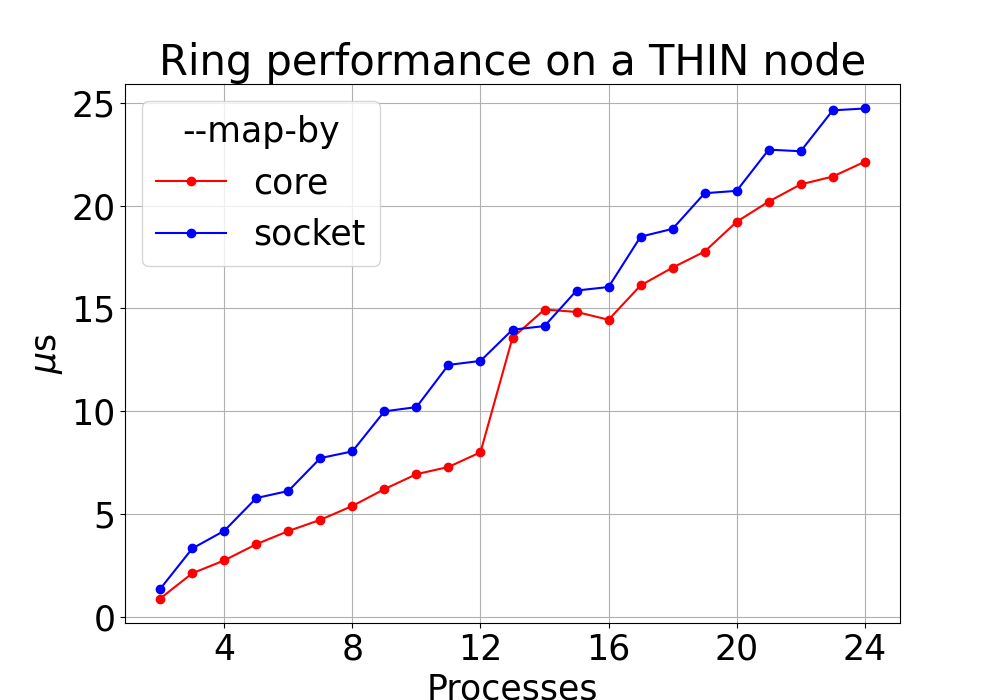
\includegraphics[width=\textwidth]{ring/fig.png}
    \caption{The script (written in C++) has been run multiple times ($\sim$ 10000) on a THIN node. Output was disabled via a compiler flag while taking times, in order to avoid polluting measurements.}
    \label{fig:ring_performance}
\end{figure}

\subsubsection{Analysis}
In Figure \ref{fig:ring_performance} we report the performance of \texttt{ring.cpp} for varying number of processors. We expect an approximately linear growth, since the addition of a new process introduces a new step in the ring (and therefore two more input and two output messages for each process).

The time is taken for two values of the parameter \texttt{--map-by}, namely \texttt{core} and \texttt{socket}. As expected the \texttt{--map-by core} case outperforms the other one until \texttt{P=13}. As soon as this threshold is passed two new communication channels are created between a process from \texttt{socket0} and a process from \texttt{socket1} (i.e. bewteen \texttt{rank11} and \texttt{rank12}, and between \texttt{rankP-1} and \texttt{rank0}), which is more costly than the communications we had in the region in the left part of the figure. This observation explains the steep increase in the execution time from 12 to 13 processes. However the evolution of the time recovers its linearity after the central region.

As you can see in the figure, the time taken by the \texttt{--map-by socket} case increases significantly only when the number of processors increases by 2, and is therefore slightly non-linear. For instance, when $P=7$ and $P=8$ the script takes $\sim$ 7.5 $\mu$s, but when $P=9$ it takes $\sim$10 $\mu$s. This is due to the fact that the mapping we chose for this case maps a process to \texttt{socket0} or \texttt{socket1} depending on its \texttt{rank}. Therefore the communication between \texttt{rank0} and \texttt{rankP-1} becomes more costly (i.e. involves two different sockets) only when \texttt{rankP-1} is located on \texttt{socket1}, which happens once for each two processes added.

\subsection{Matrix-Matrix addition}
The original formulation of this exercise led to an inefficient solution for the following reason: sending rectangular sub-blocks extracted from the matrix to each process required a copy in the general case, since in most cases we do not have the required cells in a contiguous array (\texttt{MPI\_Scatterv} allows to increase slightly the number of treatable cases, but still does not solve the general problem). Therefore we need to copy the matrix into a temporary buffer (in which blocks are stored contiguously) before calling \texttt{MPI\_Scatter}; in the end then we need to "reverse" the operation from another buffer populated with \texttt{MPI\_Gather}. However this annihilates the computational time we saved introducing MPI in the equation.

For this reason we dropped the comparison of different 1D/2D/3D topologies, and studied the \emph{strong scalability} of the summation of two 3D matrices with $P$ processes. We use \texttt{MPI\_Scatter} to send $P$ slices of size $N/P$, one for each process. Note that those slices are not blocks in the sense designated in the assignment statement: in a 3D space we could visualize them as faces of the cube (moving along the first axis). These faces may not be complete, and more than one face may be sent to each process depending on $P$ and $N$.

\textbf{Note}: I also implemented a solution for the problem which follows closely the original statement of the problem, and am able to produce it in a matter of minutes if requested.

\subsection{Experimental results}
\begin{figure}[b!]
    \centering
    \includegraphics[width=\textwidth]{matrix/time.png}
    \caption{Time measured for the addition of two 3D matrices (size $2400\times 100\times 100$). In the image we highlighted the incidence of communication time on the total time (black dotted line). The straight line at 0.05 seconds is the time it took to run the serial version of the addition (no communication).}
    \label{fig:matrix_performance}
\end{figure}

We may approximate the total time taken by the parallel implementation of the 3D matrices addition in the following way (keeping the size of the matrix fixed at $2400\times 100\times 100$):
\begin{gather}\label{eq:matrix_time_equation}
    T(P) = T_s(P) + T_\text{add}(P) + T_g(P)
\end{gather}
Where $T_s(P), T_g(P)$ are respectively the time taken by \texttt{MPI\_Scatter} and \texttt{MPI\_Gather} on $P$ processors, while $T_\text{add}(P)$ is the time taken by the summation of the portion of matrix sent to one of the $P$ processors (which may be considered approximately equal for all the processors). Obviously $T_s(1) = T_g(1) = 0$.

In Figure \ref{fig:matrix_performance} we show the contribution of each component to the total time (red dotted line). $T_\text{add}$ is the vertical distance in the plot between the total time and the communication time (black dotted line). As you can see $T_\text{add}$ is the smallest contribution, and is monotonically decreasing as expected.

By contrast, $T_s$ behaves in an unexpected way. It would make sense that the time taken by the two calls to \texttt{MPI\_Scatter} (one for each matrix to sum) increases linearly on the number of processes. However this is not the case in the left region of the plot, while we have an approximately linear relation in the right part. This probably happens due to the fact that \texttt{MPI\_Scatter} behaves in different ways depending on the number of processes and on the size of the message to send. In some cases \texttt{MPI\_Scatter} builds a binomial tree (having the root process as its root). Then the root process sends a portion of the buffer to each of its child nodes. The operation then is carried out recursively, until each process has the expected portion of the buffer.

\subsection{Conclusions}
It is clear from Figure \ref{fig:matrix_performance} that the problem scales very badly due to the unbalance between communication time and the time taken for solving the actual sub-portion of the problem (i.e. the computation of the addition of the block assigned to one of the $P$ processes). In fact the serial case ($P=1$) clearly outperforms the parallel cases.

\begin{figure}[t!]
    \centering
    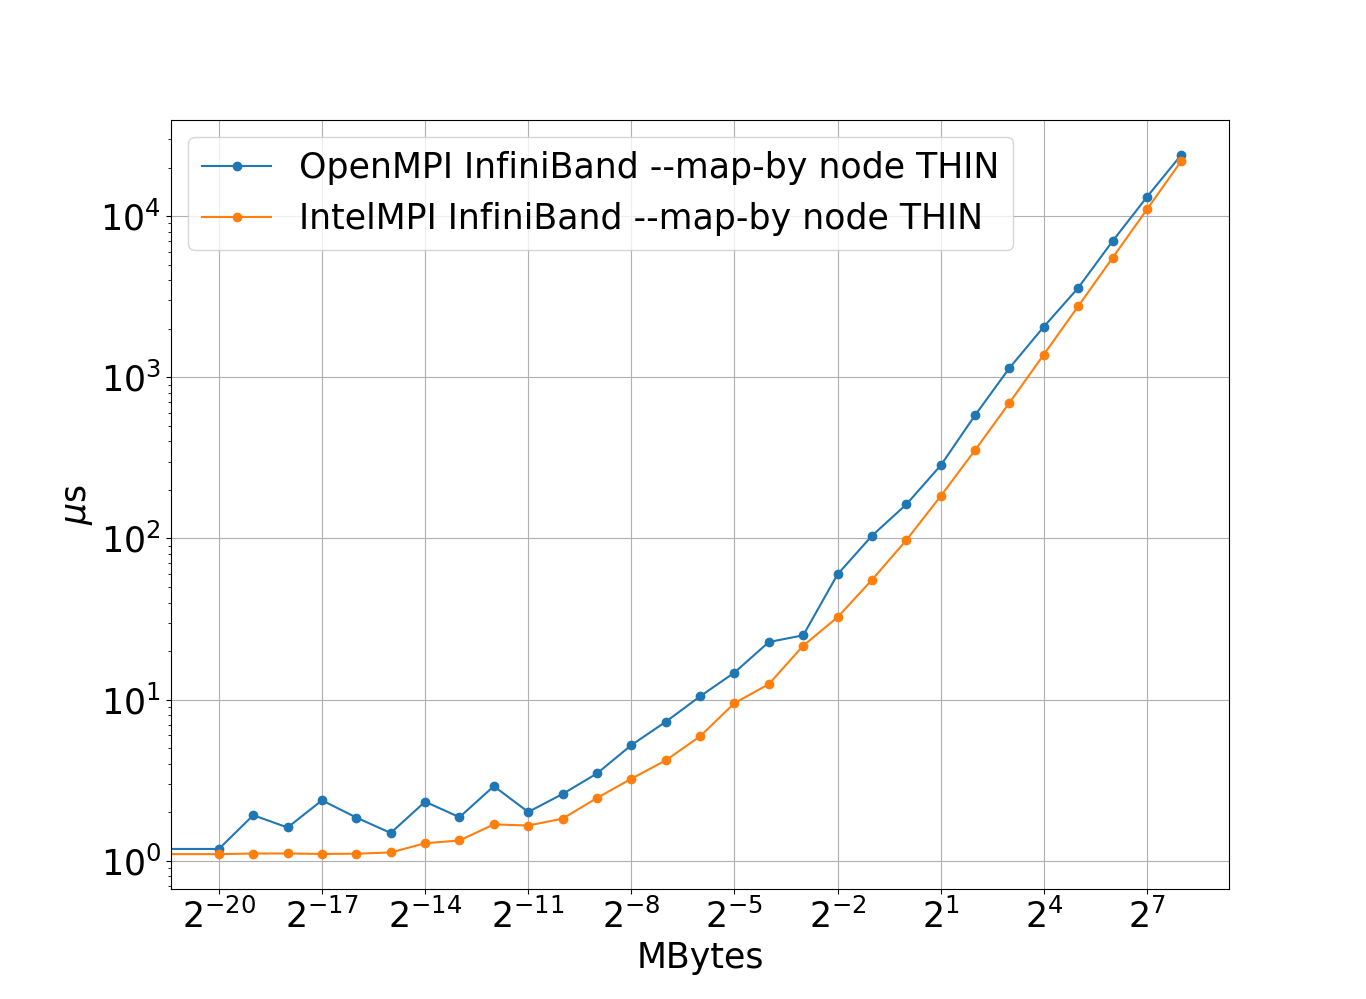
\includegraphics[width=\textwidth]{benchmark/intel_vs_ompi_node.png}
    \caption{Comparison of the time measured during the \emph{PingPong} benchmark using IntelMPI and OpenMPI, \emph{InfiniBand}, on two THIN nodes.}
    \label{fig:ompi_vs_intel}
\end{figure}

\section{Measure MPI point to point performance}
In this section we briefly disucss and present the results obtained with the \emph{PingPong} benchmark on Orfeo. The banchmark has been ran on multiple kind of nodes and networks, and against different implementations of MPI. Due to the variability that usually occurs in two consecutive runs of the benchmark we repeated each experiment 1000 times, and averaged the results element-wise.

\begin{figure}[b!]
    $$
        \begin{array}{c | c | c} \hline
            & \text{OpenMPI} & \text{IntelMPI} \\ \hline
            \hline
            \text{Core} & 0.2 \mu \text{s}  & 0.23 \mu \text{s} \\ \hline
            \text{Socket} & 0.4 \mu \text{s}  & 0.42 \mu \text{s} \\ \hline
            \text{Node} & 1.58 \mu \text{s}  & 1.08 \mu \text{s} \\ \hline
        \end{array}
    $$
    \caption{Latency computed using the simplified linear network module in OpenMPI and IntelMPI (using \emph{InfiniBand}, on THIN nodes).}
    \label{tab:lat_ompi_intel}
\end{figure}

\begin{figure}[t!]
    \centering
    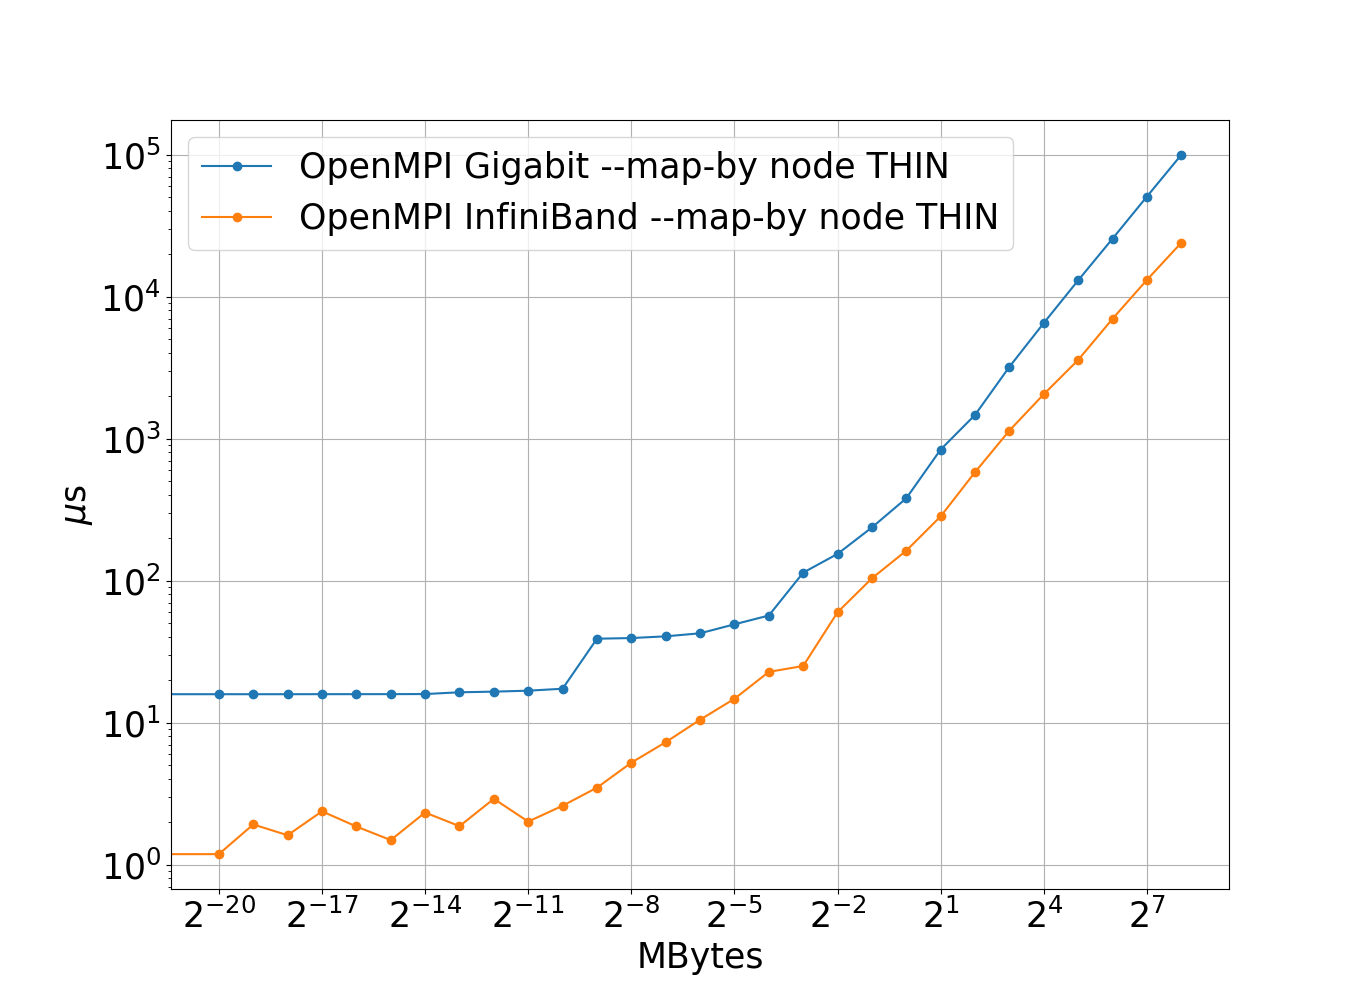
\includegraphics[width=\textwidth]{benchmark/infi_vs_giga_node.png}
    \caption{Comparison of the time measured with the \emph{PingPong} benchmark using InfiniBand and Gigabit network with OpenMPI, on two THIN nodes.}
    \label{fig:infi_vs_giga}
\end{figure}

\begin{figure}[t]
    \centering
    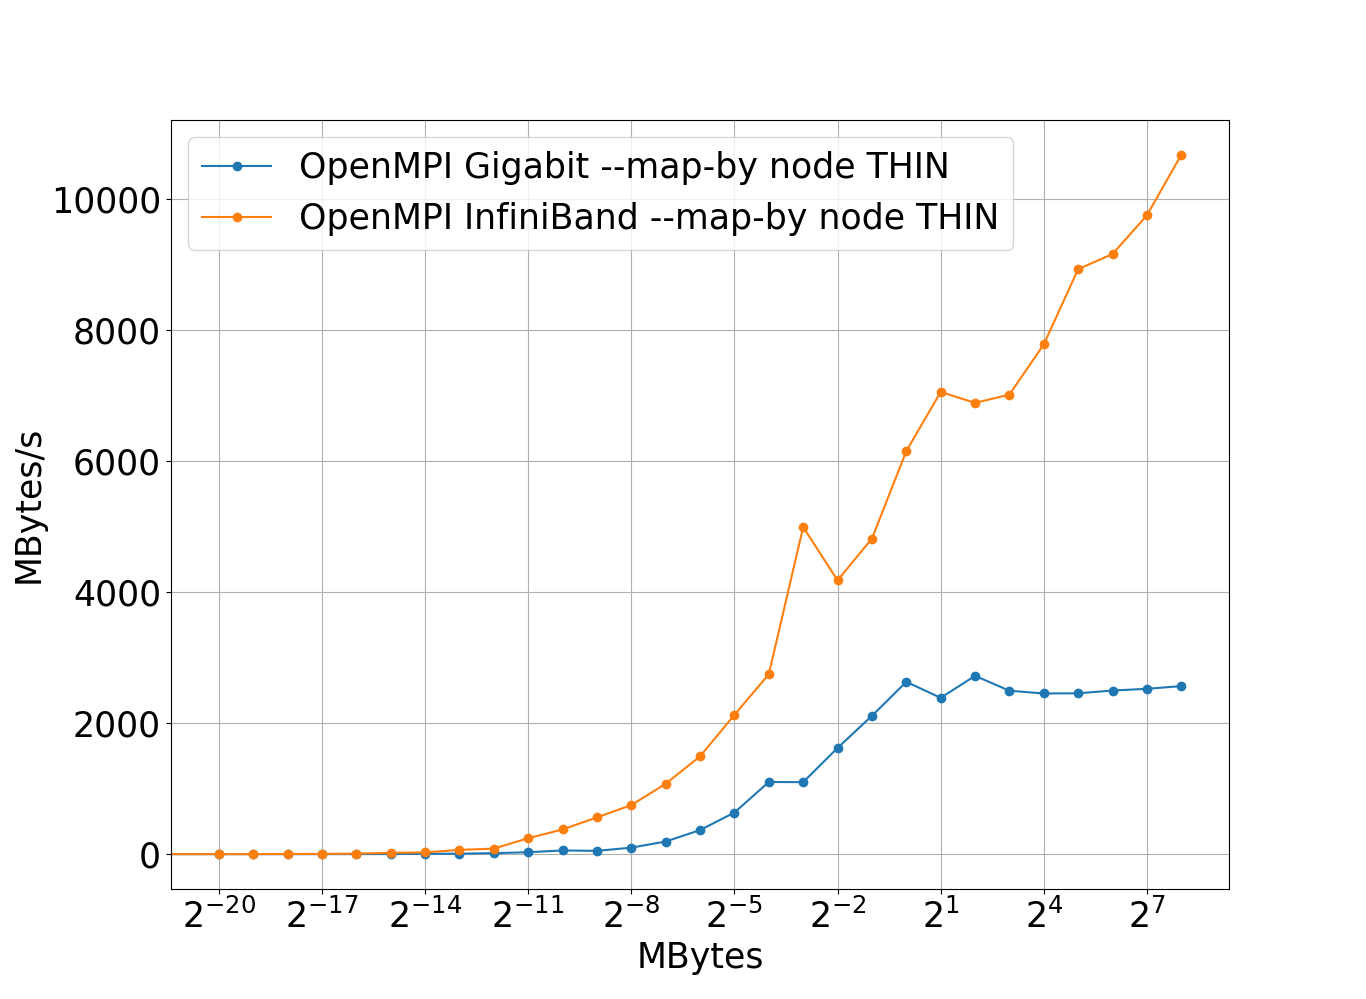
\includegraphics[width=\textwidth]{benchmark/infi_vs_giga_node_bandw.png}
    \caption{Comparison of the bandwidth measured with the \emph{PingPong} benchmark using InfiniBand and Gigabit network with OpenMPI, on two THIN nodes.}
    \label{fig:infi_vs_giga_bandwidth}
\end{figure}

\subsection{Differences observed between IntelMPI and OpenMPI}
Experiments with the \emph{PingPong} benchmark have been carried out using two different implementations of MPI available on \emph{Orfeo}, namely IntelMPI and OpenMPI. The time measured for 30 messages of growing size is shown in Figure \ref{fig:ompi_vs_intel}. It is clear that the main difference is that IntelMPI looks much more stable than OpenMPI, especially in the left region. Since the region interested by this phenomenon is the one in which latency is dominant with respect to the bandwidth, we may assume that the two implementations communicate using different protocols with the network interface, thus encountering different costs in establishing the communication and sending the message.

This assumption is supported also by the latency computed using the simplified network model (Table \ref{tab:lat_ompi_intel}), which is substantially different if we switch the MPI implementation (OpenMPI: 1.58 $\mu$s, IntelMPI: 1.08 $\mu$s). As expected the asymptotic bandwidth is almost the same in the two cases.

\subsection{Differences observed between Infiniband and Gigabit}

Looking at the left region of the graph shown in Figure \ref{fig:infi_vs_giga}, we see that the latency is clearly very different in the two cases. This is most likely due to the fact that the Gigabit network performs some more controls on the communication (e.g. it verifies that the message arrives to the receiver), therefore the message needs to pass through more layers with respect to InfiniBand network. Also, InfiniBand employs several "tricks" to make the communication faster, which likely contributes to the reduced latency. For instance when using Gigabit the user of the network has to pre-process the message using its own computational resources. This does not happen with InfiniBand, since the pre-processing happens on a software module of the network.

\begin{figure}[t!]
    \centering
    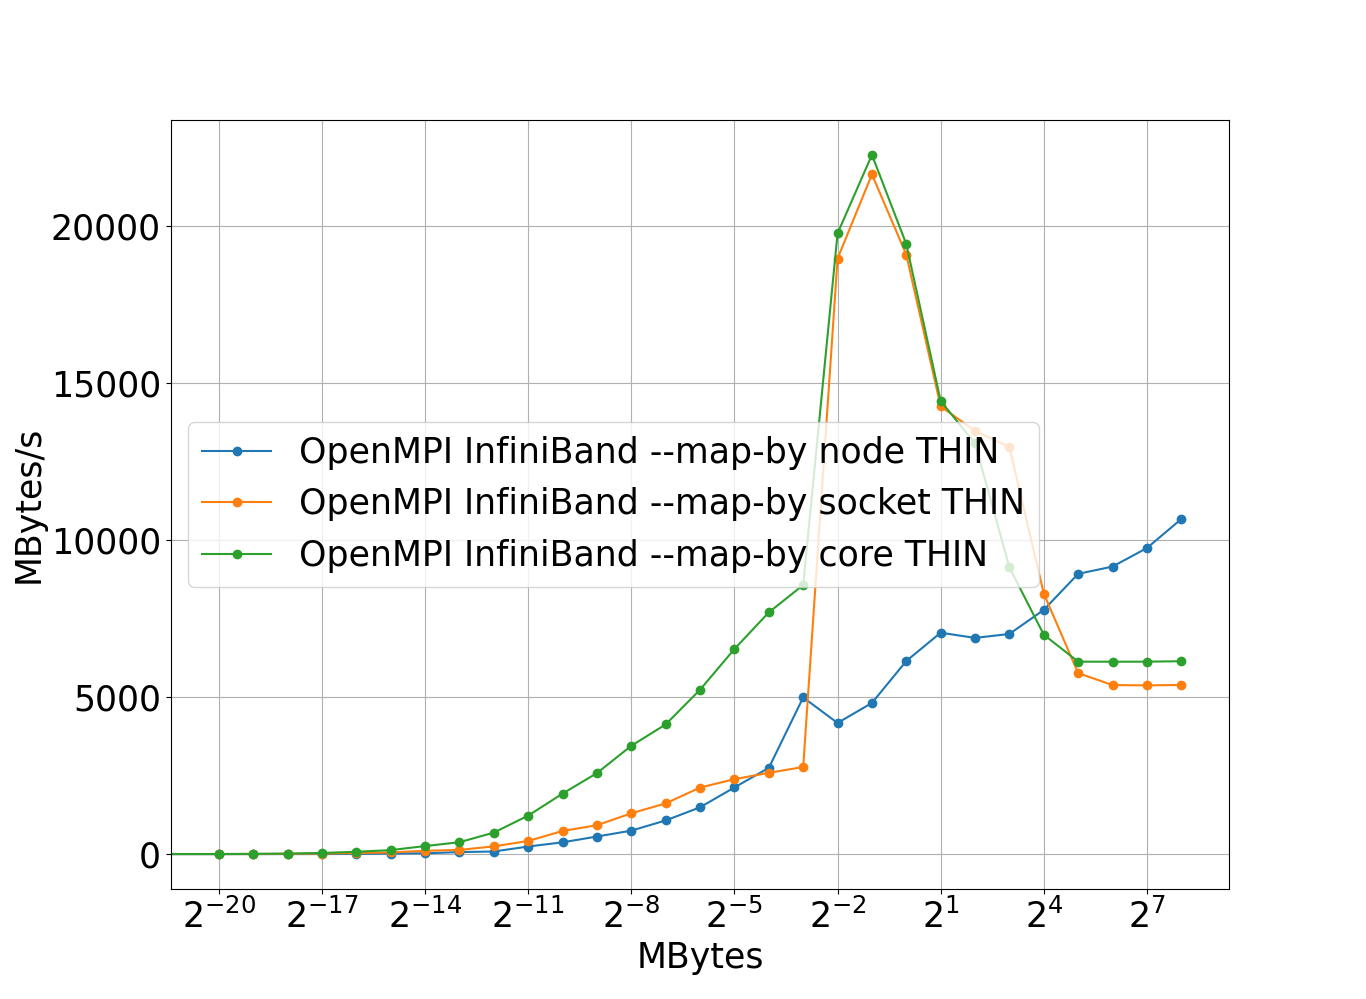
\includegraphics[width=\textwidth]{benchmark/mapby_bandwidth.png}
    \caption{Comparison of the bandwidth measured with the \emph{PingPong} benchmark using different distributions of the processes (same core, different sockets, different nodes) with OpenMPI, on THIN nodes.}
    \label{fig:mapby}
\end{figure}

Also, as you can see in Figure \ref{fig:infi_vs_giga_bandwidth}, the asymptotic bandwidth is much higher when we use InfiniBand, which is something that we could have expected before-hand.

\subsection{Other observations}

No substantial differences have been observed between THIN and GPU nodes, using both IntelMPI and OpenMPI.

As expected, the model for network performance is able to approximate the time needed to deliver a message from one process to another, as long as the size of the message is:
\begin{itemize}
    \item In the region where latency dominates the communication time;
    \item In the region where bandwidth dominates the communication time.
\end{itemize}
In the middle of these two regions the results produced using the model are not completely coherent with those measured with the benchmark.

It is interesting to observe that in general the measured asymptotic bandwidth is higher when the processes live in different nodes, with respect to the bandwidth we measured when the processes are on the same node. However the maximum bandwidth achieved is reached only in the latter case, but this does not coincide with asymptotic bandwidth as you can see in Figure \ref{fig:mapby} (in the figure the maximum bandwidth is reached when the message size is exactly 1 MByte). An hypothesis to explain this fact is that this happens due to how the message is delivered in the two cases:
\begin{itemize}
    \item When the processes live in different nodes, the message is delivered using InfiniBand network, which results in the asymptotic bandwidth observed above;
    \item When the processes live in the same node the message is delivered using the shared layers of cache (we have more shared layers if the processes are in the same socket, see the case \texttt{--map-by core} in Figure \ref{fig:mapby}).
\end{itemize}
The parts of the graphs in which we see a drop in the bandwidth, if this hypothesis is correct, are the regions in which the current message size does not fit into the cache level which was used up to that moment, therefore the time needed to transfer the message from now on is higher. Asymptotically, the message does not fit into any cache level.

\newpage
\section{Compare performance observed against performance model for Jacobi solver}
\begin{figure}[b!]
    \makebox[\textwidth][c]{
        $
        \begin{array}{c | c | c | c | c | c | c | c | c | c | c} \hline
            N  & Nx & Ny & Nz & k & C(L,N)  & T_c(L,N) &     \tilde{P}(L,N) & P(L,N) & \frac{P(1)*N}{\tilde{P}(L,N)} & \frac{P(1)*N}{P(L,N)} \\ \hline
            \hline
            1  & 1  & 1  & 1  & \texttt{n/a} & \texttt{n/a}  & \texttt{n/a}  & \texttt{n/a} & 113.423  &             1       & 1           \\ \hline
            4  & 2  & 2  & 1  &  4  & 87.891  &  0.014   &    453.264     & 409.965  &             1.001             &         1.107         \\ \hline
            8  & 2  & 2  & 2  &  6  & 131.836 &  0.022   &    906.101     & 809.103  &             1.001             &         1.121         \\ \hline
            12 & 3  & 2  & 2  &  6  & 131.836 &  0.022   &    1359.151    & 1187.816 &             1.001             &         1.146         \\ \hline
        \end{array}
        $
        }
    \caption{One thin node, \texttt{--map-by core}, latency: 0.19 $\mu$s, bandwidth: 6095 MB/s.}
\end{figure}


\begin{figure}[t!]
    \makebox[\textwidth][c]{
        $
        \begin{array}{c | c | c | c | c | c | c | c | c | c | c} \hline
            N  & Nx & Ny & Nz & k & C(L,N)  & T_c(L,N) &     \tilde{P}(L,N) & P(L,N) & \frac{P(1)*N}{\tilde{P}(L,N)} & \frac{P(1)*N}{P(L,N)} \\ \hline
            \hline
            1  & 1  & 1  & 1  & \texttt{n/a} & \texttt{n/a}  & \texttt{n/a}  & \texttt{n/a} & 113.423  &             1       & 1            \\ \hline
            4  & 2  & 2  & 1  &  4  & 87.891  &  0.017   &    453.201     & 410.274  &             1.001             &         1.106         \\ \hline
            8  & 2  & 2  & 2  &  6  & 131.836 &  0.025   &    905.910     & 811.076  &             1.002             &         1.119         \\ \hline
            12 & 3  & 2  & 2  &  6  & 131.836 &  0.025   &    1358.865    & 1213.535 &             1.002             &         1.122         \\ \hline
        \end{array}
        $
        }
    \caption{One thin node, \texttt{--map-by socket}, latency: 0.4 $\mu$s, bandwidth: 5307 MB/s.}
\end{figure}

We discuss briefly the results in the four cases taken into account (one thin node with different kinds of process mapping, two thin nodes, one GPU node with hyperthreading enabled). In the tables we show the following quantities:
\begin{itemize}
    \item $N, N_x, N_y, N_z$: respectively the total number of processes, the number of processes along the first, second and third axis;
    \item $k$: the number of axes such that the number of processors along that axis is different than one, multiplied by two;
    \item $C(L,N)$[MBytes]: the maximum data volume which transferrable on each node nework link;
    \item $T_c(L,N)$: the time it takes to communicate the halo on average;
    \item $\tilde{P}(L,N)$[MLUP/s]: MLUP per second predicted by the model, represents the number of grid cells treated per unit of time;
    \item $P(L,N)$[MLUP/s]: MLUP per second measured on Orfeo.
\end{itemize}

We also show the predicted and measured weak scalability in the last two columns. Predicted quantities are highlighted with a "tilde", therefore $\tilde(P)(L,N)$ represents the predicted number of MLUP/s.

It is clear that the model is able to recognize the evolution of the function of interest in most cases, except for the case in which we use a GPU node with hyperthreading enabled. We may theorize that the problem in this case is the fact that the model is very simple and does not take into account the effects of using hyperthreading, which also determine a very bad scalability.

However, the model overestimates $P(L,N)$, which then results in an overestimation of weak scalability (which you can see in the second to last column of our tables). Since the model "looks reasonable", and since the contribution given by the application of Jacobi's algorithms is definitely constant as the number of processors increase (and almost equal for all the processors), we may assume that the problem is inside the communication time component. Since latency has very little influence in our case, due to the size of the halos to be passed across the processes, we may theorize that the problem resides in an overestimation of the bandwidth of the machines in which we run the Jacobi solver.

\begin{figure}[h!]
    \makebox[\textwidth][c]{
        $
        \begin{array}{c | c | c | c | c | c | c | c | c | c | c} \hline
            N  & Nx & Ny & Nz & k & C(L,N)  & T_c(L,N) &     \tilde{P}(L,N) & P(L,N) & \frac{P(1)*N}{\tilde{P}(L,N)} & \frac{P(1)*N}{P(L,N)} \\ \hline
            \hline
            1  & 1  & 1  & 1  & \texttt{n/a} & \texttt{n/a}  & \texttt{n/a}  & \texttt{n/a} & 113.423  &             1       & 1            \\ \hline
            12 & 3  & 2  & 2  &  6  & 131.836 &  0.012   &    1359.980    & 1213.068 &             1.001             &         1.122         \\ \hline
            24 & 4  & 3  & 2  &  6  & 131.836 &  0.012   &    2719.959    & 2413.654 &             1.001             &         1.128         \\ \hline
            48 & 4  & 4  & 3  &  6  & 131.836 &  0.012   &    5439.919    & 4546.634 &             1.001             &         1.197         \\ \hline
        \end{array}
        $
        }
    \caption{Two thin nodes, latency: 1.58 $\mu$s, bandwidth: 10670 MB/s.}
\end{figure}


\begin{figure}[h!]
    \makebox[\textwidth][c]{
        $
        \begin{array}{c | c | c | c | c | c | c | c | c | c | c} \hline
            N  & Nx & Ny & Nz & k & C(L,N)  & T_c(L,N) &     \tilde{P}(L,N) & P(L,N) & \frac{P(1)*N}{\tilde{P}(L,N)} & \frac{P(1)*N}{P(L,N)} \\ \hline
            \hline
            1  & 1  & 1  & 1  & \texttt{n/a} & \texttt{n/a}  & \texttt{n/a}  & \texttt{n/a} & 78.269 &             1       & 1      \\ \hline
            12 & 3  & 2  & 2  &  6  & 131.836 &   0.03   &    937.958     & 817.657  &             1.001             &         1.149         \\ \hline
            24 & 4  & 3  & 2  &  6  & 131.836 &   0.03   &    1875.917    & 1390.156 &             1.001             &         1.351         \\ \hline
            48 & 4  & 4  & 3  &  6  & 131.836 &   0.03   &    3751.833    & 1441.930 &             1.001             &         2.605         \\ \hline
        \end{array}
        $
        }
    \caption{GPU node, hyperthreading enabled, latency: 0.43 $\mu$s, bandwidth: 4415 MB/s.}
\end{figure}

\end{document}
